\documentclass[twoside]{book}

% Packages required by doxygen
\usepackage{fixltx2e}
\usepackage{calc}
\usepackage{doxygen}
\usepackage[export]{adjustbox} % also loads graphicx
\usepackage{graphicx}
\usepackage[utf8]{inputenc}
\usepackage{makeidx}
\usepackage{multicol}
\usepackage{multirow}
\PassOptionsToPackage{warn}{textcomp}
\usepackage{textcomp}
\usepackage[nointegrals]{wasysym}
\usepackage[table]{xcolor}

% Font selection
\usepackage[T1]{fontenc}
\usepackage[scaled=.90]{helvet}
\usepackage{courier}
\usepackage{amssymb}
\usepackage{sectsty}
\renewcommand{\familydefault}{\sfdefault}
\allsectionsfont{%
  \fontseries{bc}\selectfont%
  \color{darkgray}%
}
\renewcommand{\DoxyLabelFont}{%
  \fontseries{bc}\selectfont%
  \color{darkgray}%
}
\newcommand{\+}{\discretionary{\mbox{\scriptsize$\hookleftarrow$}}{}{}}

% Page & text layout
\usepackage{geometry}
\geometry{%
  a4paper,%
  top=2.5cm,%
  bottom=2.5cm,%
  left=2.5cm,%
  right=2.5cm%
}
\tolerance=750
\hfuzz=15pt
\hbadness=750
\setlength{\emergencystretch}{15pt}
\setlength{\parindent}{0cm}
\setlength{\parskip}{3ex plus 2ex minus 2ex}
\makeatletter
\renewcommand{\paragraph}{%
  \@startsection{paragraph}{4}{0ex}{-1.0ex}{1.0ex}{%
    \normalfont\normalsize\bfseries\SS@parafont%
  }%
}
\renewcommand{\subparagraph}{%
  \@startsection{subparagraph}{5}{0ex}{-1.0ex}{1.0ex}{%
    \normalfont\normalsize\bfseries\SS@subparafont%
  }%
}
\makeatother

% Headers & footers
\usepackage{fancyhdr}
\pagestyle{fancyplain}
\fancyhead[LE]{\fancyplain{}{\bfseries\thepage}}
\fancyhead[CE]{\fancyplain{}{}}
\fancyhead[RE]{\fancyplain{}{\bfseries\leftmark}}
\fancyhead[LO]{\fancyplain{}{\bfseries\rightmark}}
\fancyhead[CO]{\fancyplain{}{}}
\fancyhead[RO]{\fancyplain{}{\bfseries\thepage}}
\fancyfoot[LE]{\fancyplain{}{}}
\fancyfoot[CE]{\fancyplain{}{}}
\fancyfoot[RE]{\fancyplain{}{\bfseries\scriptsize Generated by Doxygen }}
\fancyfoot[LO]{\fancyplain{}{\bfseries\scriptsize Generated by Doxygen }}
\fancyfoot[CO]{\fancyplain{}{}}
\fancyfoot[RO]{\fancyplain{}{}}
\renewcommand{\footrulewidth}{0.4pt}
\renewcommand{\chaptermark}[1]{%
  \markboth{#1}{}%
}
\renewcommand{\sectionmark}[1]{%
  \markright{\thesection\ #1}%
}

% Indices & bibliography
\usepackage{natbib}
\usepackage[titles]{tocloft}
\setcounter{tocdepth}{3}
\setcounter{secnumdepth}{5}
\makeindex

% Hyperlinks (required, but should be loaded last)
\usepackage{ifpdf}
\ifpdf
  \usepackage[pdftex,pagebackref=true]{hyperref}
\else
  \usepackage[ps2pdf,pagebackref=true]{hyperref}
\fi
\hypersetup{%
  colorlinks=true,%
  linkcolor=blue,%
  citecolor=blue,%
  unicode%
}

% Custom commands
\newcommand{\clearemptydoublepage}{%
  \newpage{\pagestyle{empty}\cleardoublepage}%
}

\usepackage{caption}
\captionsetup{labelsep=space,justification=centering,font={bf},singlelinecheck=off,skip=4pt,position=top}

%===== C O N T E N T S =====

\begin{document}

% Titlepage & ToC
\hypersetup{pageanchor=false,
             bookmarksnumbered=true,
             pdfencoding=unicode
            }
\pagenumbering{alph}
\begin{titlepage}
\vspace*{7cm}
\begin{center}%
{\Large Heis }\\
\vspace*{1cm}
{\large Generated by Doxygen 1.8.13}\\
\end{center}
\end{titlepage}
\clearemptydoublepage
\pagenumbering{roman}
\tableofcontents
\clearemptydoublepage
\pagenumbering{arabic}
\hypersetup{pageanchor=true}

%--- Begin generated contents ---
\chapter{Data Structure Index}
\section{Data Structures}
Here are the data structures with brief descriptions\+:\begin{DoxyCompactList}
\item\contentsline{section}{\hyperlink{structElevator}{Elevator} \\*Struct representing the elevator cabine }{\pageref{structElevator}}{}
\end{DoxyCompactList}

\chapter{File Index}
\section{File List}
Here is a list of all documented files with brief descriptions\+:\begin{DoxyCompactList}
\item\contentsline{section}{source/{\bfseries el\+Utils.\+c} }{\pageref{elUtils_8c}}{}
\item\contentsline{section}{source/\hyperlink{elUtils_8h}{el\+Utils.\+h} \\*Utilities for the elevator system }{\pageref{elUtils_8h}}{}
\item\contentsline{section}{source/{\bfseries F\+S\+M.\+c} }{\pageref{FSM_8c}}{}
\item\contentsline{section}{source/\hyperlink{FSM_8h}{F\+S\+M.\+h} \\*Final state machine for elevator }{\pageref{FSM_8h}}{}
\item\contentsline{section}{source/\hyperlink{hardware_8h}{hardware.\+h} \\*Driver for the elevator hardware }{\pageref{hardware_8h}}{}
\item\contentsline{section}{source/{\bfseries main.\+c} }{\pageref{main_8c}}{}
\item\contentsline{section}{source/{\bfseries timer.\+c} }{\pageref{timer_8c}}{}
\item\contentsline{section}{source/\hyperlink{timer_8h}{timer.\+h} \\*Utilities for time management }{\pageref{timer_8h}}{}
\end{DoxyCompactList}

\chapter{Data Structure Documentation}
\hypertarget{structElevator}{}\section{Elevator Struct Reference}
\label{structElevator}\index{Elevator@{Elevator}}


Struct representing the elevator cabine.  




{\ttfamily \#include $<$el\+Utils.\+h$>$}

\subsection*{Data Fields}
\begin{DoxyCompactItemize}
\item 
\mbox{\Hypertarget{structElevator_ae52fd8b99f21d281c58194ab1734ddc5}\label{structElevator_ae52fd8b99f21d281c58194ab1734ddc5}} 
Flore\+Type {\bfseries floor}
\item 
\mbox{\Hypertarget{structElevator_a5bc377c8e13b288861cc2e67866e9a5c}\label{structElevator_a5bc377c8e13b288861cc2e67866e9a5c}} 
\hyperlink{hardware_8h_a2167c399a24df296afc432bcb88228af}{Hardware\+Movement} {\bfseries direction}
\item 
\mbox{\Hypertarget{structElevator_a92134b58a13b924fba94f145b9475b72}\label{structElevator_a92134b58a13b924fba94f145b9475b72}} 
int {\bfseries elevator\+\_\+queue} \mbox{[}4\mbox{]}\mbox{[}3\mbox{]}
\item 
\mbox{\Hypertarget{structElevator_ab576b8da1f8fcb53cfdaef5019fac0a6}\label{structElevator_ab576b8da1f8fcb53cfdaef5019fac0a6}} 
Elevator\+State {\bfseries state}
\end{DoxyCompactItemize}


\subsection{Detailed Description}
Struct representing the elevator cabine. 

Definition at line 26 of file el\+Utils.\+h.



The documentation for this struct was generated from the following file\+:\begin{DoxyCompactItemize}
\item 
source/\hyperlink{elUtils_8h}{el\+Utils.\+h}\end{DoxyCompactItemize}

\chapter{File Documentation}
\hypertarget{elUtils_8h}{}\section{source/el\+Utils.h File Reference}
\label{elUtils_8h}\index{source/el\+Utils.\+h@{source/el\+Utils.\+h}}


Utilities for the elevator system.  


{\ttfamily \#include \char`\"{}hardware.\+h\char`\"{}}\newline
Include dependency graph for el\+Utils.\+h\+:
\nopagebreak
\begin{figure}[H]
\begin{center}
\leavevmode
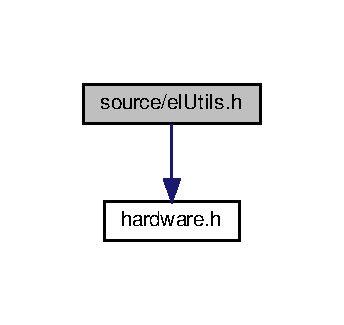
\includegraphics[width=165pt]{elUtils_8h__incl}
\end{center}
\end{figure}
This graph shows which files directly or indirectly include this file\+:
\nopagebreak
\begin{figure}[H]
\begin{center}
\leavevmode
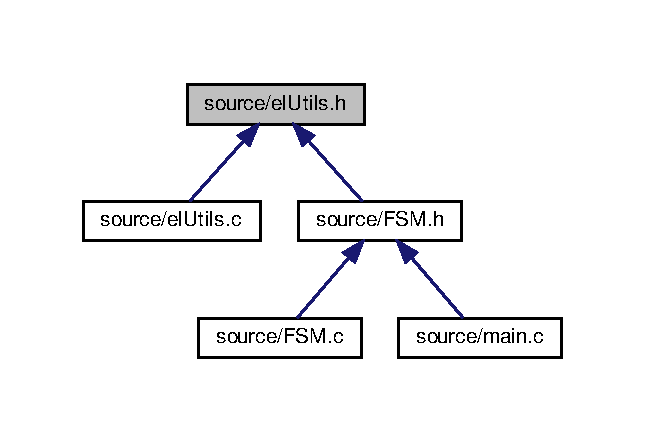
\includegraphics[width=310pt]{elUtils_8h__dep__incl}
\end{center}
\end{figure}
\subsection*{Data Structures}
\begin{DoxyCompactItemize}
\item 
struct \hyperlink{structElevator}{Elevator}
\begin{DoxyCompactList}\small\item\em Struct representing the elevator cabine. \end{DoxyCompactList}\end{DoxyCompactItemize}
\subsection*{Enumerations}
\begin{DoxyCompactItemize}
\item 
\mbox{\Hypertarget{elUtils_8h_ada8a6679b36fc4f29442334494afb588}\label{elUtils_8h_ada8a6679b36fc4f29442334494afb588}} 
enum {\bfseries Elevator\+State} \{ {\bfseries I\+D\+EL}, 
{\bfseries M\+O\+V\+I\+NG}, 
{\bfseries D\+O\+O\+R\+\_\+\+O\+P\+EN}
 \}
\item 
\mbox{\Hypertarget{elUtils_8h_ace2259f62830a9f6ccaad5ab7ab9e80a}\label{elUtils_8h_ace2259f62830a9f6ccaad5ab7ab9e80a}} 
enum {\bfseries Flore\+Type} \{ {\bfseries F\+L\+O\+O\+R1}, 
{\bfseries F\+L\+O\+O\+R2}, 
{\bfseries F\+L\+O\+O\+R3}, 
{\bfseries F\+L\+O\+O\+R4}
 \}
\end{DoxyCompactItemize}
\subsection*{Functions}
\begin{DoxyCompactItemize}
\item 
\mbox{\Hypertarget{elUtils_8h_a70e1a2dcbe6d12a160f3a4881cb7fec7}\label{elUtils_8h_a70e1a2dcbe6d12a160f3a4881cb7fec7}} 
void \hyperlink{elUtils_8h_a70e1a2dcbe6d12a160f3a4881cb7fec7}{el\+Utils\+\_\+init\+\_\+elevator} (struct \hyperlink{structElevator}{Elevator} $\ast$e)
\begin{DoxyCompactList}\small\item\em An extension of {\ttfamily hardware\+\_\+init} Commands the elevator to move to first floor and go to idel. \end{DoxyCompactList}\item 
\mbox{\Hypertarget{elUtils_8h_a153460c061c812ffaba8a0ce445366ae}\label{elUtils_8h_a153460c061c812ffaba8a0ce445366ae}} 
void \hyperlink{elUtils_8h_a153460c061c812ffaba8a0ce445366ae}{el\+Utils\+\_\+clear\+\_\+order\+\_\+queue} (struct \hyperlink{structElevator}{Elevator} $\ast$e)
\begin{DoxyCompactList}\small\item\em Sets all elements of elevator queue matrix to null. \end{DoxyCompactList}\item 
\hyperlink{hardware_8h_a2167c399a24df296afc432bcb88228af}{Hardware\+Movement} \hyperlink{elUtils_8h_aedcb7d91e8e7d7c39f46284f4ed7b29d}{el\+Utils\+\_\+set\+\_\+direction\+\_\+for\+\_\+idel} (struct \hyperlink{structElevator}{Elevator} $\ast$e)
\begin{DoxyCompactList}\small\item\em Polls the elevator queue matrix for orders. \end{DoxyCompactList}\item 
\mbox{\Hypertarget{elUtils_8h_aea35fc89a330e0d1d5d3b4956b848c93}\label{elUtils_8h_aea35fc89a330e0d1d5d3b4956b848c93}} 
void \hyperlink{elUtils_8h_aea35fc89a330e0d1d5d3b4956b848c93}{el\+Utils\+\_\+add\+\_\+new\+\_\+order} (struct \hyperlink{structElevator}{Elevator} $\ast$e)
\begin{DoxyCompactList}\small\item\em Adds new order to elevator queue matrix. \end{DoxyCompactList}\item 
\mbox{\Hypertarget{elUtils_8h_a1c53ead73831f33955438edb4c4f11be}\label{elUtils_8h_a1c53ead73831f33955438edb4c4f11be}} 
void \hyperlink{elUtils_8h_a1c53ead73831f33955438edb4c4f11be}{el\+Utils\+\_\+clear\+\_\+order} (struct \hyperlink{structElevator}{Elevator} $\ast$e)
\begin{DoxyCompactList}\small\item\em Clears all orders at the current floor from elevator queue matrix. \end{DoxyCompactList}\item 
int \hyperlink{elUtils_8h_ae49f864115bee644796c935b4ee73531}{el\+Utils\+\_\+read\+\_\+new\+\_\+floor} (struct \hyperlink{structElevator}{Elevator} $\ast$e)
\begin{DoxyCompactList}\small\item\em An extension of {\ttfamily hardware\+\_\+read\+\_\+floor\+\_\+sensor}. \end{DoxyCompactList}\item 
int \hyperlink{elUtils_8h_a88de4a1a7ba9aece0bc4e4372c9f0d18}{should\+\_\+i\+\_\+stop} (struct \hyperlink{structElevator}{Elevator} $\ast$e)
\begin{DoxyCompactList}\small\item\em Polls the elevator queue matrix for orders at current floor. \end{DoxyCompactList}\item 
int \hyperlink{elUtils_8h_af8663d757e6f99d175bba29739f979ab}{should\+\_\+i\+\_\+continue} (struct \hyperlink{structElevator}{Elevator} $\ast$e)
\begin{DoxyCompactList}\small\item\em Polls the elevator queue matrix for orders in the same direction as the movement of the cabine. \end{DoxyCompactList}\item 
int \hyperlink{elUtils_8h_acb8f067362006373b6c8a7cfdffb4278}{should\+\_\+i\+\_\+turn} (struct \hyperlink{structElevator}{Elevator} $\ast$e)
\begin{DoxyCompactList}\small\item\em Polls the elevator queue matrix for orders in the opposite direction of the movement of the cabine. \end{DoxyCompactList}\end{DoxyCompactItemize}


\subsection{Detailed Description}
Utilities for the elevator system. 



\subsection{Function Documentation}
\mbox{\Hypertarget{elUtils_8h_ae49f864115bee644796c935b4ee73531}\label{elUtils_8h_ae49f864115bee644796c935b4ee73531}} 
\index{el\+Utils.\+h@{el\+Utils.\+h}!el\+Utils\+\_\+read\+\_\+new\+\_\+floor@{el\+Utils\+\_\+read\+\_\+new\+\_\+floor}}
\index{el\+Utils\+\_\+read\+\_\+new\+\_\+floor@{el\+Utils\+\_\+read\+\_\+new\+\_\+floor}!el\+Utils.\+h@{el\+Utils.\+h}}
\subsubsection{\texorpdfstring{el\+Utils\+\_\+read\+\_\+new\+\_\+floor()}{elUtils\_read\_new\_floor()}}
{\footnotesize\ttfamily int el\+Utils\+\_\+read\+\_\+new\+\_\+floor (\begin{DoxyParamCaption}\item[{struct \hyperlink{structElevator}{Elevator} $\ast$}]{e }\end{DoxyParamCaption})}



An extension of {\ttfamily hardware\+\_\+read\+\_\+floor\+\_\+sensor}. 

\begin{DoxyReturn}{Returns}
1 on arrival at new floor, 0 otherwise. 
\end{DoxyReturn}


Definition at line 78 of file el\+Utils.\+c.

\mbox{\Hypertarget{elUtils_8h_aedcb7d91e8e7d7c39f46284f4ed7b29d}\label{elUtils_8h_aedcb7d91e8e7d7c39f46284f4ed7b29d}} 
\index{el\+Utils.\+h@{el\+Utils.\+h}!el\+Utils\+\_\+set\+\_\+direction\+\_\+for\+\_\+idel@{el\+Utils\+\_\+set\+\_\+direction\+\_\+for\+\_\+idel}}
\index{el\+Utils\+\_\+set\+\_\+direction\+\_\+for\+\_\+idel@{el\+Utils\+\_\+set\+\_\+direction\+\_\+for\+\_\+idel}!el\+Utils.\+h@{el\+Utils.\+h}}
\subsubsection{\texorpdfstring{el\+Utils\+\_\+set\+\_\+direction\+\_\+for\+\_\+idel()}{elUtils\_set\_direction\_for\_idel()}}
{\footnotesize\ttfamily \hyperlink{hardware_8h_a2167c399a24df296afc432bcb88228af}{Hardware\+Movement} el\+Utils\+\_\+set\+\_\+direction\+\_\+for\+\_\+idel (\begin{DoxyParamCaption}\item[{struct \hyperlink{structElevator}{Elevator} $\ast$}]{e }\end{DoxyParamCaption})}



Polls the elevator queue matrix for orders. 

\begin{DoxyReturn}{Returns}
Direction for movement according to first order. 
\end{DoxyReturn}


Definition at line 36 of file el\+Utils.\+c.

\mbox{\Hypertarget{elUtils_8h_af8663d757e6f99d175bba29739f979ab}\label{elUtils_8h_af8663d757e6f99d175bba29739f979ab}} 
\index{el\+Utils.\+h@{el\+Utils.\+h}!should\+\_\+i\+\_\+continue@{should\+\_\+i\+\_\+continue}}
\index{should\+\_\+i\+\_\+continue@{should\+\_\+i\+\_\+continue}!el\+Utils.\+h@{el\+Utils.\+h}}
\subsubsection{\texorpdfstring{should\+\_\+i\+\_\+continue()}{should\_i\_continue()}}
{\footnotesize\ttfamily int should\+\_\+i\+\_\+continue (\begin{DoxyParamCaption}\item[{struct \hyperlink{structElevator}{Elevator} $\ast$}]{e }\end{DoxyParamCaption})}



Polls the elevator queue matrix for orders in the same direction as the movement of the cabine. 

\begin{DoxyReturn}{Returns}
1 on success, 0 otherwise. 
\end{DoxyReturn}


Definition at line 99 of file el\+Utils.\+c.

\mbox{\Hypertarget{elUtils_8h_a88de4a1a7ba9aece0bc4e4372c9f0d18}\label{elUtils_8h_a88de4a1a7ba9aece0bc4e4372c9f0d18}} 
\index{el\+Utils.\+h@{el\+Utils.\+h}!should\+\_\+i\+\_\+stop@{should\+\_\+i\+\_\+stop}}
\index{should\+\_\+i\+\_\+stop@{should\+\_\+i\+\_\+stop}!el\+Utils.\+h@{el\+Utils.\+h}}
\subsubsection{\texorpdfstring{should\+\_\+i\+\_\+stop()}{should\_i\_stop()}}
{\footnotesize\ttfamily int should\+\_\+i\+\_\+stop (\begin{DoxyParamCaption}\item[{struct \hyperlink{structElevator}{Elevator} $\ast$}]{e }\end{DoxyParamCaption})}



Polls the elevator queue matrix for orders at current floor. 

\begin{DoxyReturn}{Returns}
1 if there is an order from inside the cabin, or outside in the same direction as the movement of the cabine. 
\end{DoxyReturn}


Definition at line 85 of file el\+Utils.\+c.

\mbox{\Hypertarget{elUtils_8h_acb8f067362006373b6c8a7cfdffb4278}\label{elUtils_8h_acb8f067362006373b6c8a7cfdffb4278}} 
\index{el\+Utils.\+h@{el\+Utils.\+h}!should\+\_\+i\+\_\+turn@{should\+\_\+i\+\_\+turn}}
\index{should\+\_\+i\+\_\+turn@{should\+\_\+i\+\_\+turn}!el\+Utils.\+h@{el\+Utils.\+h}}
\subsubsection{\texorpdfstring{should\+\_\+i\+\_\+turn()}{should\_i\_turn()}}
{\footnotesize\ttfamily int should\+\_\+i\+\_\+turn (\begin{DoxyParamCaption}\item[{struct \hyperlink{structElevator}{Elevator} $\ast$}]{e }\end{DoxyParamCaption})}



Polls the elevator queue matrix for orders in the opposite direction of the movement of the cabine. 

\begin{DoxyReturn}{Returns}
1 on success, 0 otherwise. 
\end{DoxyReturn}


Definition at line 121 of file el\+Utils.\+c.


\hypertarget{FSM_8h}{}\section{source/\+F\+SM.h File Reference}
\label{FSM_8h}\index{source/\+F\+S\+M.\+h@{source/\+F\+S\+M.\+h}}


Final state machine for elevator.  


{\ttfamily \#include \char`\"{}el\+Utils.\+h\char`\"{}}\newline
Include dependency graph for F\+S\+M.\+h\+:
\nopagebreak
\begin{figure}[H]
\begin{center}
\leavevmode
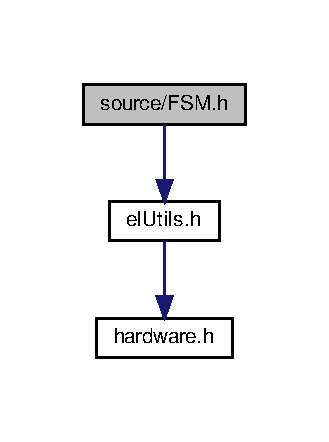
\includegraphics[width=158pt]{FSM_8h__incl}
\end{center}
\end{figure}
This graph shows which files directly or indirectly include this file\+:
\nopagebreak
\begin{figure}[H]
\begin{center}
\leavevmode
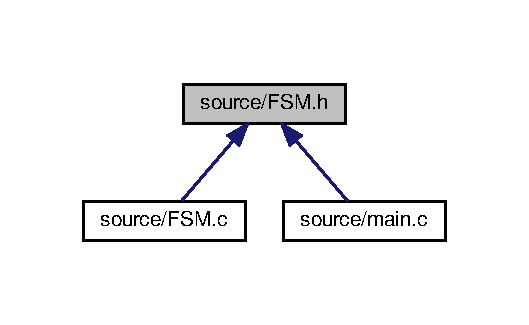
\includegraphics[width=254pt]{FSM_8h__dep__incl}
\end{center}
\end{figure}
\subsection*{Functions}
\begin{DoxyCompactItemize}
\item 
\mbox{\Hypertarget{FSM_8h_aec770b37493303bbe8335efcd039fec3}\label{FSM_8h_aec770b37493303bbe8335efcd039fec3}} 
void \hyperlink{FSM_8h_aec770b37493303bbe8335efcd039fec3}{F\+S\+M\+\_\+stop} (struct \hyperlink{structElevator}{Elevator} $\ast$e)
\begin{DoxyCompactList}\small\item\em Executes if {\ttfamily hardware\+\_\+read\+\_\+stop\+\_\+signal}, is set high. Clears order queue and all oder lights, and sets elevator state to idel. \end{DoxyCompactList}\item 
\mbox{\Hypertarget{FSM_8h_a571a2533ed77fbda3f06ead707a25953}\label{FSM_8h_a571a2533ed77fbda3f06ead707a25953}} 
void \hyperlink{FSM_8h_a571a2533ed77fbda3f06ead707a25953}{F\+S\+M\+\_\+new\+\_\+order} (struct \hyperlink{structElevator}{Elevator} $\ast$e)
\begin{DoxyCompactList}\small\item\em Adds new order to elevator order matrix. If the state of the elevator is idel. The elevator determines the proper direction based on whether it is between or at a floor. \end{DoxyCompactList}\item 
\mbox{\Hypertarget{FSM_8h_af7e2e41595037350a9e488a017753e4a}\label{FSM_8h_af7e2e41595037350a9e488a017753e4a}} 
void \hyperlink{FSM_8h_af7e2e41595037350a9e488a017753e4a}{F\+S\+M\+\_\+time\+\_\+out} (struct \hyperlink{structElevator}{Elevator} $\ast$e)
\begin{DoxyCompactList}\small\item\em Executes at experation of timer. Determines if the cabine should continue or change direction by {\ttfamily should\+\_\+i\+\_\+continue}, and {\ttfamily should\+\_\+i\+\_\+turn} respectively in that order. If not, the elevator goes to idel. For every case the cabin state parameters are set accordingly. \end{DoxyCompactList}\item 
\mbox{\Hypertarget{FSM_8h_a572aed55033d0bf29f6ecd2a07aec134}\label{FSM_8h_a572aed55033d0bf29f6ecd2a07aec134}} 
void \hyperlink{FSM_8h_a572aed55033d0bf29f6ecd2a07aec134}{F\+S\+M\+\_\+arrived\+\_\+new\+\_\+floor} (struct \hyperlink{structElevator}{Elevator} $\ast$e)
\begin{DoxyCompactList}\small\item\em Executes at arrival of new floor. Determines if the cabine should stop by {\ttfamily should\+\_\+i\+\_\+stop} and sets the cabin state parameters accordingly. Either the cabine stops and dispatches an order, or it continues in the same direction. \end{DoxyCompactList}\item 
\mbox{\Hypertarget{FSM_8h_aac6904f37d0e94bf7e2c4a7dc2c8d628}\label{FSM_8h_aac6904f37d0e94bf7e2c4a7dc2c8d628}} 
void \hyperlink{FSM_8h_aac6904f37d0e94bf7e2c4a7dc2c8d628}{F\+S\+M\+\_\+run} ()
\begin{DoxyCompactList}\small\item\em Final state machine of the system. Checks for the triggers and executes the above functions accordingly. \end{DoxyCompactList}\end{DoxyCompactItemize}


\subsection{Detailed Description}
Final state machine for elevator. 


\hypertarget{hardware_8h}{}\section{source/hardware.h File Reference}
\label{hardware_8h}\index{source/hardware.\+h@{source/hardware.\+h}}


Driver for the elevator hardware.  


This graph shows which files directly or indirectly include this file\+:
\nopagebreak
\begin{figure}[H]
\begin{center}
\leavevmode
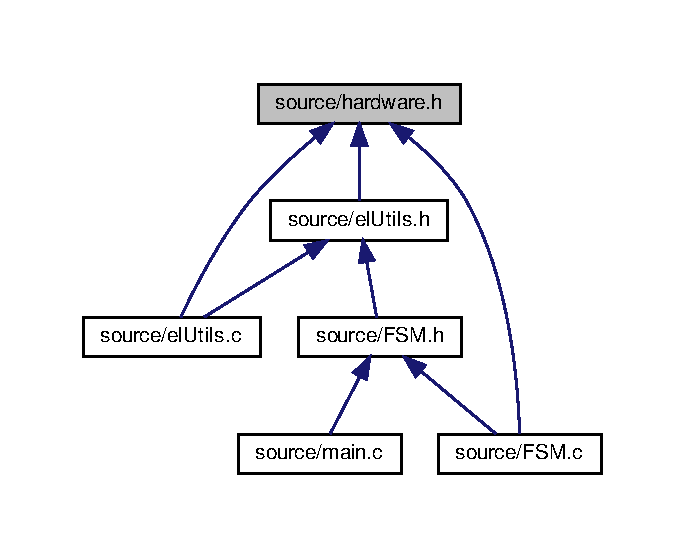
\includegraphics[width=329pt]{hardware_8h__dep__incl}
\end{center}
\end{figure}
\subsection*{Macros}
\begin{DoxyCompactItemize}
\item 
\mbox{\Hypertarget{hardware_8h_ae9e42615eade15633bd8c03b7a271a00}\label{hardware_8h_ae9e42615eade15633bd8c03b7a271a00}} 
\#define {\bfseries H\+A\+R\+D\+W\+A\+R\+E\+\_\+\+N\+U\+M\+B\+E\+R\+\_\+\+O\+F\+\_\+\+F\+L\+O\+O\+RS}~4
\item 
\mbox{\Hypertarget{hardware_8h_ac476fea44244889602251233c8747a83}\label{hardware_8h_ac476fea44244889602251233c8747a83}} 
\#define {\bfseries H\+A\+R\+D\+W\+A\+R\+E\+\_\+\+N\+U\+M\+B\+E\+R\+\_\+\+O\+F\+\_\+\+O\+R\+D\+E\+R\+\_\+\+T\+Y\+P\+ES}~3
\end{DoxyCompactItemize}
\subsection*{Enumerations}
\begin{DoxyCompactItemize}
\item 
\mbox{\Hypertarget{hardware_8h_a2167c399a24df296afc432bcb88228af}\label{hardware_8h_a2167c399a24df296afc432bcb88228af}} 
enum \hyperlink{hardware_8h_a2167c399a24df296afc432bcb88228af}{Hardware\+Movement} \{ {\bfseries H\+A\+R\+D\+W\+A\+R\+E\+\_\+\+M\+O\+V\+E\+M\+E\+N\+T\+\_\+\+UP}, 
{\bfseries H\+A\+R\+D\+W\+A\+R\+E\+\_\+\+M\+O\+V\+E\+M\+E\+N\+T\+\_\+\+S\+T\+OP}, 
{\bfseries H\+A\+R\+D\+W\+A\+R\+E\+\_\+\+M\+O\+V\+E\+M\+E\+N\+T\+\_\+\+D\+O\+WN}
 \}\begin{DoxyCompactList}\small\item\em Movement type used in {\ttfamily hardware\+\_\+command\+\_\+movement}. \end{DoxyCompactList}
\item 
\mbox{\Hypertarget{hardware_8h_a796a8de8ce0ae769d7dbd3327a7bdbe7}\label{hardware_8h_a796a8de8ce0ae769d7dbd3327a7bdbe7}} 
enum \hyperlink{hardware_8h_a796a8de8ce0ae769d7dbd3327a7bdbe7}{Hardware\+Order} \{ {\bfseries H\+A\+R\+D\+W\+A\+R\+E\+\_\+\+O\+R\+D\+E\+R\+\_\+\+UP}, 
{\bfseries H\+A\+R\+D\+W\+A\+R\+E\+\_\+\+O\+R\+D\+E\+R\+\_\+\+I\+N\+S\+I\+DE}, 
{\bfseries H\+A\+R\+D\+W\+A\+R\+E\+\_\+\+O\+R\+D\+E\+R\+\_\+\+D\+O\+WN}
 \}\begin{DoxyCompactList}\small\item\em Order type used in {\ttfamily hardware\+\_\+read\+\_\+order} and in {\ttfamily hardware\+\_\+command\+\_\+order\+\_\+light}. \end{DoxyCompactList}
\end{DoxyCompactItemize}
\subsection*{Functions}
\begin{DoxyCompactItemize}
\item 
int \hyperlink{hardware_8h_a054b8fb8768311d46be58d6a4890d771}{hardware\+\_\+init} ()
\begin{DoxyCompactList}\small\item\em Initializes the elevator control hardware. Must be called once before other calls to the elevator hardware driver. \end{DoxyCompactList}\item 
void \hyperlink{hardware_8h_a01de081ef0510a111053c18cd31afa27}{hardware\+\_\+command\+\_\+movement} (\hyperlink{hardware_8h_a2167c399a24df296afc432bcb88228af}{Hardware\+Movement} movement)
\begin{DoxyCompactList}\small\item\em Commands the elevator to either move up or down, or commands it to halt. \end{DoxyCompactList}\item 
int \hyperlink{hardware_8h_a4a77b27c86675c00b513db3445966804}{hardware\+\_\+read\+\_\+stop\+\_\+signal} ()
\begin{DoxyCompactList}\small\item\em Polls the hardware for the current stop signal. \end{DoxyCompactList}\item 
int \hyperlink{hardware_8h_a459fe57a3ee4bc2a28e8a15b2ab14c2d}{hardware\+\_\+read\+\_\+obstruction\+\_\+signal} ()
\begin{DoxyCompactList}\small\item\em Polls the hardware for the current obstruction signal. \end{DoxyCompactList}\item 
int \hyperlink{hardware_8h_ab048489e6302bb5604aad753f2d7d501}{hardware\+\_\+read\+\_\+floor\+\_\+sensor} (int floor)
\begin{DoxyCompactList}\small\item\em Polls the floor sensor for the given {\ttfamily floor}. \end{DoxyCompactList}\item 
int \hyperlink{hardware_8h_a87917f3aa093fb46ca821a400d011ee8}{hardware\+\_\+read\+\_\+order} (int floor, \hyperlink{hardware_8h_a796a8de8ce0ae769d7dbd3327a7bdbe7}{Hardware\+Order} order\+\_\+type)
\begin{DoxyCompactList}\small\item\em Polls the hardware for the status of orders from floor {\ttfamily floor} of type {\ttfamily order\+\_\+type}. \end{DoxyCompactList}\item 
void \hyperlink{hardware_8h_a80d99ddaa8e7b58c9a88b60ea553c1b6}{hardware\+\_\+command\+\_\+door\+\_\+open} (int door\+\_\+open)
\begin{DoxyCompactList}\small\item\em Commands the hardware to open-\/ or close the elevator door. \end{DoxyCompactList}\item 
void \hyperlink{hardware_8h_a407a6ec035ba357de6aa0fbe55501d1e}{hardware\+\_\+command\+\_\+floor\+\_\+indicator\+\_\+on} (int floor)
\begin{DoxyCompactList}\small\item\em Commands the hardware to turn on the floor indicator for {\ttfamily floor}. All indicators all mutually exclusive; other indicator lights will turn off. \end{DoxyCompactList}\item 
void \hyperlink{hardware_8h_aa75b3ac17f72b25946414f48d0063a10}{hardware\+\_\+command\+\_\+stop\+\_\+light} (int on)
\begin{DoxyCompactList}\small\item\em Sets the light in the panel stop button. \end{DoxyCompactList}\item 
void \hyperlink{hardware_8h_aa9b33faa52f0ec5b614d3e7dc05be140}{hardware\+\_\+command\+\_\+order\+\_\+light} (int floor, \hyperlink{hardware_8h_a796a8de8ce0ae769d7dbd3327a7bdbe7}{Hardware\+Order} order\+\_\+type, int on)
\begin{DoxyCompactList}\small\item\em Sets the light in a button corresponding to an order of type {\ttfamily order\+\_\+type}, at floor {\ttfamily floor}. \end{DoxyCompactList}\item 
\mbox{\Hypertarget{hardware_8h_ade8cba977d7db232f54b9faafcad6a3f}\label{hardware_8h_ade8cba977d7db232f54b9faafcad6a3f}} 
void \hyperlink{hardware_8h_ade8cba977d7db232f54b9faafcad6a3f}{hardware\+\_\+command\+\_\+clear\+\_\+all\+\_\+order\+\_\+lights} ()
\begin{DoxyCompactList}\small\item\em clears all order lights \end{DoxyCompactList}\item 
int \hyperlink{hardware_8h_aaad35e60b5c1152daa2aba559c82a829}{hardware\+\_\+read\+\_\+all\+\_\+orders} ()
\begin{DoxyCompactList}\small\item\em Polls the hardware for the status of orders from all floors. \end{DoxyCompactList}\item 
int \hyperlink{hardware_8h_ad3c3fee158a845c2fbf7012bbb7eb700}{hardware\+\_\+read\+\_\+all\+\_\+floor\+\_\+sensors} ()
\begin{DoxyCompactList}\small\item\em Polls the floor sensor for all floors. \end{DoxyCompactList}\item 
int \hyperlink{hardware_8h_a938f6f945f81e0b645c05cb908e8dbdb}{hardware\+\_\+read\+\_\+current\+\_\+floor} ()
\end{DoxyCompactItemize}


\subsection{Detailed Description}
Driver for the elevator hardware. 

Kolbjørn Austreng 

\subsection{Function Documentation}
\mbox{\Hypertarget{hardware_8h_a80d99ddaa8e7b58c9a88b60ea553c1b6}\label{hardware_8h_a80d99ddaa8e7b58c9a88b60ea553c1b6}} 
\index{hardware.\+h@{hardware.\+h}!hardware\+\_\+command\+\_\+door\+\_\+open@{hardware\+\_\+command\+\_\+door\+\_\+open}}
\index{hardware\+\_\+command\+\_\+door\+\_\+open@{hardware\+\_\+command\+\_\+door\+\_\+open}!hardware.\+h@{hardware.\+h}}
\subsubsection{\texorpdfstring{hardware\+\_\+command\+\_\+door\+\_\+open()}{hardware\_command\_door\_open()}}
{\footnotesize\ttfamily void hardware\+\_\+command\+\_\+door\+\_\+open (\begin{DoxyParamCaption}\item[{int}]{door\+\_\+open }\end{DoxyParamCaption})}



Commands the hardware to open-\/ or close the elevator door. 


\begin{DoxyParams}{Parameters}
{\em door\+\_\+open} & A truthy value (non-\/zero) to open the door; 0 to close. \\
\hline
\end{DoxyParams}
\mbox{\Hypertarget{hardware_8h_a407a6ec035ba357de6aa0fbe55501d1e}\label{hardware_8h_a407a6ec035ba357de6aa0fbe55501d1e}} 
\index{hardware.\+h@{hardware.\+h}!hardware\+\_\+command\+\_\+floor\+\_\+indicator\+\_\+on@{hardware\+\_\+command\+\_\+floor\+\_\+indicator\+\_\+on}}
\index{hardware\+\_\+command\+\_\+floor\+\_\+indicator\+\_\+on@{hardware\+\_\+command\+\_\+floor\+\_\+indicator\+\_\+on}!hardware.\+h@{hardware.\+h}}
\subsubsection{\texorpdfstring{hardware\+\_\+command\+\_\+floor\+\_\+indicator\+\_\+on()}{hardware\_command\_floor\_indicator\_on()}}
{\footnotesize\ttfamily void hardware\+\_\+command\+\_\+floor\+\_\+indicator\+\_\+on (\begin{DoxyParamCaption}\item[{int}]{floor }\end{DoxyParamCaption})}



Commands the hardware to turn on the floor indicator for {\ttfamily floor}. All indicators all mutually exclusive; other indicator lights will turn off. 


\begin{DoxyParams}{Parameters}
{\em floor} & Floor to turn on the indicator for.\\
\hline
\end{DoxyParams}
\begin{DoxyWarning}{Warning}
Owing to peculiarities in the hardware construction, there will always be one indicator active. 
\end{DoxyWarning}
\mbox{\Hypertarget{hardware_8h_a01de081ef0510a111053c18cd31afa27}\label{hardware_8h_a01de081ef0510a111053c18cd31afa27}} 
\index{hardware.\+h@{hardware.\+h}!hardware\+\_\+command\+\_\+movement@{hardware\+\_\+command\+\_\+movement}}
\index{hardware\+\_\+command\+\_\+movement@{hardware\+\_\+command\+\_\+movement}!hardware.\+h@{hardware.\+h}}
\subsubsection{\texorpdfstring{hardware\+\_\+command\+\_\+movement()}{hardware\_command\_movement()}}
{\footnotesize\ttfamily void hardware\+\_\+command\+\_\+movement (\begin{DoxyParamCaption}\item[{\hyperlink{hardware_8h_a2167c399a24df296afc432bcb88228af}{Hardware\+Movement}}]{movement }\end{DoxyParamCaption})}



Commands the elevator to either move up or down, or commands it to halt. 


\begin{DoxyParams}{Parameters}
{\em movement} & Commanded movement. \\
\hline
\end{DoxyParams}
\mbox{\Hypertarget{hardware_8h_aa9b33faa52f0ec5b614d3e7dc05be140}\label{hardware_8h_aa9b33faa52f0ec5b614d3e7dc05be140}} 
\index{hardware.\+h@{hardware.\+h}!hardware\+\_\+command\+\_\+order\+\_\+light@{hardware\+\_\+command\+\_\+order\+\_\+light}}
\index{hardware\+\_\+command\+\_\+order\+\_\+light@{hardware\+\_\+command\+\_\+order\+\_\+light}!hardware.\+h@{hardware.\+h}}
\subsubsection{\texorpdfstring{hardware\+\_\+command\+\_\+order\+\_\+light()}{hardware\_command\_order\_light()}}
{\footnotesize\ttfamily void hardware\+\_\+command\+\_\+order\+\_\+light (\begin{DoxyParamCaption}\item[{int}]{floor,  }\item[{\hyperlink{hardware_8h_a796a8de8ce0ae769d7dbd3327a7bdbe7}{Hardware\+Order}}]{order\+\_\+type,  }\item[{int}]{on }\end{DoxyParamCaption})}



Sets the light in a button corresponding to an order of type {\ttfamily order\+\_\+type}, at floor {\ttfamily floor}. 


\begin{DoxyParams}{Parameters}
{\em floor} & The floor of the order indicator. \\
\hline
{\em order\+\_\+type} & The type of order. \\
\hline
{\em on} & A truthy value (non-\/zero) to turn the light on; 0 to turn it off. \\
\hline
\end{DoxyParams}
\mbox{\Hypertarget{hardware_8h_aa75b3ac17f72b25946414f48d0063a10}\label{hardware_8h_aa75b3ac17f72b25946414f48d0063a10}} 
\index{hardware.\+h@{hardware.\+h}!hardware\+\_\+command\+\_\+stop\+\_\+light@{hardware\+\_\+command\+\_\+stop\+\_\+light}}
\index{hardware\+\_\+command\+\_\+stop\+\_\+light@{hardware\+\_\+command\+\_\+stop\+\_\+light}!hardware.\+h@{hardware.\+h}}
\subsubsection{\texorpdfstring{hardware\+\_\+command\+\_\+stop\+\_\+light()}{hardware\_command\_stop\_light()}}
{\footnotesize\ttfamily void hardware\+\_\+command\+\_\+stop\+\_\+light (\begin{DoxyParamCaption}\item[{int}]{on }\end{DoxyParamCaption})}



Sets the light in the panel stop button. 


\begin{DoxyParams}{Parameters}
{\em on} & A truthy value (non-\/zero) to turn the light on; 0 to turn it off. \\
\hline
\end{DoxyParams}
\mbox{\Hypertarget{hardware_8h_a054b8fb8768311d46be58d6a4890d771}\label{hardware_8h_a054b8fb8768311d46be58d6a4890d771}} 
\index{hardware.\+h@{hardware.\+h}!hardware\+\_\+init@{hardware\+\_\+init}}
\index{hardware\+\_\+init@{hardware\+\_\+init}!hardware.\+h@{hardware.\+h}}
\subsubsection{\texorpdfstring{hardware\+\_\+init()}{hardware\_init()}}
{\footnotesize\ttfamily int hardware\+\_\+init (\begin{DoxyParamCaption}{ }\end{DoxyParamCaption})}



Initializes the elevator control hardware. Must be called once before other calls to the elevator hardware driver. 

\begin{DoxyReturn}{Returns}
0 on success. Non-\/zero for failure. 
\end{DoxyReturn}
\mbox{\Hypertarget{hardware_8h_ad3c3fee158a845c2fbf7012bbb7eb700}\label{hardware_8h_ad3c3fee158a845c2fbf7012bbb7eb700}} 
\index{hardware.\+h@{hardware.\+h}!hardware\+\_\+read\+\_\+all\+\_\+floor\+\_\+sensors@{hardware\+\_\+read\+\_\+all\+\_\+floor\+\_\+sensors}}
\index{hardware\+\_\+read\+\_\+all\+\_\+floor\+\_\+sensors@{hardware\+\_\+read\+\_\+all\+\_\+floor\+\_\+sensors}!hardware.\+h@{hardware.\+h}}
\subsubsection{\texorpdfstring{hardware\+\_\+read\+\_\+all\+\_\+floor\+\_\+sensors()}{hardware\_read\_all\_floor\_sensors()}}
{\footnotesize\ttfamily int hardware\+\_\+read\+\_\+all\+\_\+floor\+\_\+sensors (\begin{DoxyParamCaption}{ }\end{DoxyParamCaption})}



Polls the floor sensor for all floors. 

\begin{DoxyReturn}{Returns}
1 if the elevator is at any floor. 
\end{DoxyReturn}
\mbox{\Hypertarget{hardware_8h_aaad35e60b5c1152daa2aba559c82a829}\label{hardware_8h_aaad35e60b5c1152daa2aba559c82a829}} 
\index{hardware.\+h@{hardware.\+h}!hardware\+\_\+read\+\_\+all\+\_\+orders@{hardware\+\_\+read\+\_\+all\+\_\+orders}}
\index{hardware\+\_\+read\+\_\+all\+\_\+orders@{hardware\+\_\+read\+\_\+all\+\_\+orders}!hardware.\+h@{hardware.\+h}}
\subsubsection{\texorpdfstring{hardware\+\_\+read\+\_\+all\+\_\+orders()}{hardware\_read\_all\_orders()}}
{\footnotesize\ttfamily int hardware\+\_\+read\+\_\+all\+\_\+orders (\begin{DoxyParamCaption}{ }\end{DoxyParamCaption})}



Polls the hardware for the status of orders from all floors. 

\begin{DoxyReturn}{Returns}
1 if there is an order at any floor. 
\end{DoxyReturn}
\mbox{\Hypertarget{hardware_8h_a938f6f945f81e0b645c05cb908e8dbdb}\label{hardware_8h_a938f6f945f81e0b645c05cb908e8dbdb}} 
\index{hardware.\+h@{hardware.\+h}!hardware\+\_\+read\+\_\+current\+\_\+floor@{hardware\+\_\+read\+\_\+current\+\_\+floor}}
\index{hardware\+\_\+read\+\_\+current\+\_\+floor@{hardware\+\_\+read\+\_\+current\+\_\+floor}!hardware.\+h@{hardware.\+h}}
\subsubsection{\texorpdfstring{hardware\+\_\+read\+\_\+current\+\_\+floor()}{hardware\_read\_current\_floor()}}
{\footnotesize\ttfamily int hardware\+\_\+read\+\_\+current\+\_\+floor (\begin{DoxyParamCaption}{ }\end{DoxyParamCaption})}

\begin{DoxyReturn}{Returns}
an integer corresponding to current floor. 
\end{DoxyReturn}
\mbox{\Hypertarget{hardware_8h_ab048489e6302bb5604aad753f2d7d501}\label{hardware_8h_ab048489e6302bb5604aad753f2d7d501}} 
\index{hardware.\+h@{hardware.\+h}!hardware\+\_\+read\+\_\+floor\+\_\+sensor@{hardware\+\_\+read\+\_\+floor\+\_\+sensor}}
\index{hardware\+\_\+read\+\_\+floor\+\_\+sensor@{hardware\+\_\+read\+\_\+floor\+\_\+sensor}!hardware.\+h@{hardware.\+h}}
\subsubsection{\texorpdfstring{hardware\+\_\+read\+\_\+floor\+\_\+sensor()}{hardware\_read\_floor\_sensor()}}
{\footnotesize\ttfamily int hardware\+\_\+read\+\_\+floor\+\_\+sensor (\begin{DoxyParamCaption}\item[{int}]{floor }\end{DoxyParamCaption})}



Polls the floor sensor for the given {\ttfamily floor}. 


\begin{DoxyParams}{Parameters}
{\em floor} & Inquired floor.\\
\hline
\end{DoxyParams}
\begin{DoxyReturn}{Returns}
1 if the elevator is at {\ttfamily floor}, otherwise 0; 
\end{DoxyReturn}
\mbox{\Hypertarget{hardware_8h_a459fe57a3ee4bc2a28e8a15b2ab14c2d}\label{hardware_8h_a459fe57a3ee4bc2a28e8a15b2ab14c2d}} 
\index{hardware.\+h@{hardware.\+h}!hardware\+\_\+read\+\_\+obstruction\+\_\+signal@{hardware\+\_\+read\+\_\+obstruction\+\_\+signal}}
\index{hardware\+\_\+read\+\_\+obstruction\+\_\+signal@{hardware\+\_\+read\+\_\+obstruction\+\_\+signal}!hardware.\+h@{hardware.\+h}}
\subsubsection{\texorpdfstring{hardware\+\_\+read\+\_\+obstruction\+\_\+signal()}{hardware\_read\_obstruction\_signal()}}
{\footnotesize\ttfamily int hardware\+\_\+read\+\_\+obstruction\+\_\+signal (\begin{DoxyParamCaption}{ }\end{DoxyParamCaption})}



Polls the hardware for the current obstruction signal. 

\begin{DoxyReturn}{Returns}
1 if the obstruction signal is high; 0 if it is low. 
\end{DoxyReturn}
\mbox{\Hypertarget{hardware_8h_a87917f3aa093fb46ca821a400d011ee8}\label{hardware_8h_a87917f3aa093fb46ca821a400d011ee8}} 
\index{hardware.\+h@{hardware.\+h}!hardware\+\_\+read\+\_\+order@{hardware\+\_\+read\+\_\+order}}
\index{hardware\+\_\+read\+\_\+order@{hardware\+\_\+read\+\_\+order}!hardware.\+h@{hardware.\+h}}
\subsubsection{\texorpdfstring{hardware\+\_\+read\+\_\+order()}{hardware\_read\_order()}}
{\footnotesize\ttfamily int hardware\+\_\+read\+\_\+order (\begin{DoxyParamCaption}\item[{int}]{floor,  }\item[{\hyperlink{hardware_8h_a796a8de8ce0ae769d7dbd3327a7bdbe7}{Hardware\+Order}}]{order\+\_\+type }\end{DoxyParamCaption})}



Polls the hardware for the status of orders from floor {\ttfamily floor} of type {\ttfamily order\+\_\+type}. 


\begin{DoxyParams}{Parameters}
{\em floor} & Inquired floor. \\
\hline
{\em order\+\_\+type} & \\
\hline
\end{DoxyParams}
\begin{DoxyReturn}{Returns}
1 if the combination of {\ttfamily floor} and {\ttfamily order\+\_\+type} is being requested, otherwise 0. 
\end{DoxyReturn}
\mbox{\Hypertarget{hardware_8h_a4a77b27c86675c00b513db3445966804}\label{hardware_8h_a4a77b27c86675c00b513db3445966804}} 
\index{hardware.\+h@{hardware.\+h}!hardware\+\_\+read\+\_\+stop\+\_\+signal@{hardware\+\_\+read\+\_\+stop\+\_\+signal}}
\index{hardware\+\_\+read\+\_\+stop\+\_\+signal@{hardware\+\_\+read\+\_\+stop\+\_\+signal}!hardware.\+h@{hardware.\+h}}
\subsubsection{\texorpdfstring{hardware\+\_\+read\+\_\+stop\+\_\+signal()}{hardware\_read\_stop\_signal()}}
{\footnotesize\ttfamily int hardware\+\_\+read\+\_\+stop\+\_\+signal (\begin{DoxyParamCaption}{ }\end{DoxyParamCaption})}



Polls the hardware for the current stop signal. 

\begin{DoxyReturn}{Returns}
1 if the stop signal is high; 0 if it is low. 
\end{DoxyReturn}

\hypertarget{timer_8h}{}\section{source/timer.h File Reference}
\label{timer_8h}\index{source/timer.\+h@{source/timer.\+h}}


Utilities for time management.  


This graph shows which files directly or indirectly include this file\+:
\nopagebreak
\begin{figure}[H]
\begin{center}
\leavevmode
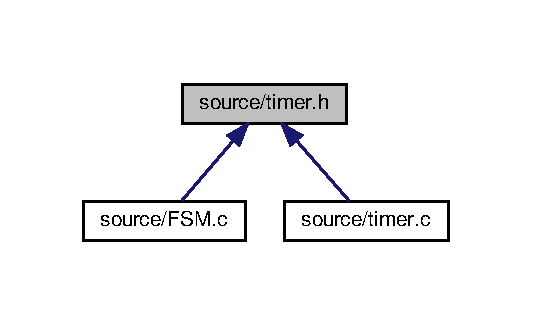
\includegraphics[width=256pt]{timer_8h__dep__incl}
\end{center}
\end{figure}
\subsection*{Functions}
\begin{DoxyCompactItemize}
\item 
\mbox{\Hypertarget{timer_8h_a161432848a326da3a1ea7765fc2bc023}\label{timer_8h_a161432848a326da3a1ea7765fc2bc023}} 
void \hyperlink{timer_8h_a161432848a326da3a1ea7765fc2bc023}{timer\+\_\+start} ()
\begin{DoxyCompactList}\small\item\em Sets global variablel end\+\_\+time in the source file to current time pluss 3 seconds. \end{DoxyCompactList}\item 
int \hyperlink{timer_8h_a8f87954693f6080c10d94bd5e65a6bee}{timer\+\_\+out} ()
\begin{DoxyCompactList}\small\item\em Check timer. \end{DoxyCompactList}\end{DoxyCompactItemize}
\subsection*{Variables}
\begin{DoxyCompactItemize}
\item 
\mbox{\Hypertarget{timer_8h_a7af890518fa05f17c8627195dfacf5d7}\label{timer_8h_a7af890518fa05f17c8627195dfacf5d7}} 
int {\bfseries timer\+\_\+enable}
\end{DoxyCompactItemize}


\subsection{Detailed Description}
Utilities for time management. 



\subsection{Function Documentation}
\mbox{\Hypertarget{timer_8h_a8f87954693f6080c10d94bd5e65a6bee}\label{timer_8h_a8f87954693f6080c10d94bd5e65a6bee}} 
\index{timer.\+h@{timer.\+h}!timer\+\_\+out@{timer\+\_\+out}}
\index{timer\+\_\+out@{timer\+\_\+out}!timer.\+h@{timer.\+h}}
\subsubsection{\texorpdfstring{timer\+\_\+out()}{timer\_out()}}
{\footnotesize\ttfamily int timer\+\_\+out (\begin{DoxyParamCaption}{ }\end{DoxyParamCaption})}



Check timer. 

\begin{DoxyReturn}{Returns}
1 if the timer has expired, 0 otherwise. 
\end{DoxyReturn}


Definition at line 13 of file timer.\+c.


%--- End generated contents ---

% Index
\backmatter
\newpage
\phantomsection
\clearemptydoublepage
\addcontentsline{toc}{chapter}{Index}
\printindex

\end{document}
